%%%%%%%%%%%%%%%%%%%%%%%%%%%%%%%%%%%%%%%%%%%%%%%%%
%%%%%%%%%%%%%%%%%%%%%%%%%%%%%%%%%%%%%%%%%%%%%%%%%

\documentclass[12pt,a4paper]{scrartcl}

%%%%%%%%%%%%%%%%%%%%%%%%%%%%%%%%%%%%%%%%%%%%%%%%%
%%%%%%%%%%%%%%%%%%%%%%%%%%%%%%%%%%%%%%%%%%%%%%%%%

\usepackage[utf8]{inputenc}
\usepackage[english]{babel}
\usepackage[T1]{fontenc}

%%%%%%%%%%%%%%%%%%%%%%%%%%%%%%%%%%%%%%%%%%%%%%%%%
%%%%%%%%%%%%%%%%%%%%%%%%%%%%%%%%%%%%%%%%%%%%%%%%%

%\usepackage{ucs}
\usepackage{amsmath}
\usepackage{amssymb}

%%%%%%%%%%%%%%%%%%%%%%%%%%%%%%%%%%%%%%%%%%%%%%%%%
%%%%%%%%%%%%%%%%%%%%%%%%%%%%%%%%%%%%%%%%%%%%%%%%%

\usepackage{graphicx}
\usepackage{tabularx,colortbl}
\usepackage{capt-of}
\usepackage{booktabs}
\usepackage{hyperref}

%%%%%%%%%%%%%%%%%%%%%%%%%%%%%%%%%%%%%%%%%%%%%%%%%
%%%%%%%%%%%%%%%%%%%%%%%%%%%%%%%%%%%%%%%%%%%%%%%%%

\usepackage{pdflscape}
\usepackage{pdfpages}

%%%%%%%%%%%%%%%%%%%%%%%%%%%%%%%%%%%%%%%%%%%%%%%%%
%%%%%%%%%%%%%%%%%%%%%%%%%%%%%%%%%%%%%%%%%%%%%%%%%

\usepackage[group-separator={,}, group-minimum-digits=3]{siunitx}
\DeclareSIUnit\basepair{bp}
\DeclareSIUnit\byte{B}

%%%%%%%%%%%%%%%%%%%%%%%%%%%%%%%%%%%%%%%%%%%%%%%%%
%%%%%%%%%%%%%%%%%%%%%%%%%%%%%%%%%%%%%%%%%%%%%%%%%

\usepackage{biocon}
\newtaxon{strain}
\newtaxastyle{WithStrain}{\taxit{\taxonfirst{!genus!.}\taxon{ !epithet!}} str. \#\taxon{!strain!}}

\newanimal{Hd}{genus=Hybsibuis,epithet=dujardini}

%%%%%%%%%%%%%%%%%%%%%%%%%%%%%%%%%%%%%%%%%%%%%%%%%
%%%%%%%%%%%%%%%%%%%%%%%%%%%%%%%%%%%%%%%%%%%%%%%%%

\usepackage{enumitem}
\setlist[enumerate]{itemsep=0mm}

%%%%%%%%%%%%%%%%%%%%%%%%%%%%%%%%%%%%%%%%%%%%%%%%%
%%%%%%%%%%%%%%%%%%%%%%%%%%%%%%%%%%%%%%%%%%%%%%%%%

\usepackage{tabularx}
\usepackage[backend=biber]{biblatex}
\addbibresource{supplement.bib}
\usepackage{rotating}
\usepackage{cleveref}
\usepackage{listings}
\lstset{basicstyle=\ttfamily\footnotesize}

%%%%%%%%%%%%%%%%%%%%%%%%%%%%%%%%%%%%%%%%%%%%%%%%%
%%%%%%%%%%%%%%%%%%%%%%%%%%%%%%%%%%%%%%%%%%%%%%%%%

\title{\Large The genome of a tardigrade - \\\large Horizontal gene transfer or bacterial contamination?}
\author{\normalsize Felix Bemm, Clemens Weiß, Jörg Schultz, Frank Förster}
\date{}

%%%%%%%%%%%%%%%%%%%%%%%%%%%%%%%%%%%%%%%%%%%%%%%%%
%%%%%%%%%%%%%%%%%%%%%%%%%%%%%%%%%%%%%%%%%%%%%%%%%

\graphicspath{{./figures/}}
\DeclareGraphicsExtensions{.pdf,.PDF,.png,.PNG,.jpg,.JPG,.jpeg,.JPEG}

%%%%%%%%%%%%%%%%%%%%%%%%%%%%%%%%%%%%%%%%%%%%%%%%%
%%%%%%%%%%%%%%%%%%%%%%%%%%%%%%%%%%%%%%%%%%%%%%%%%

\begin{document}

\maketitle

\pagebreak

\section{Figures}

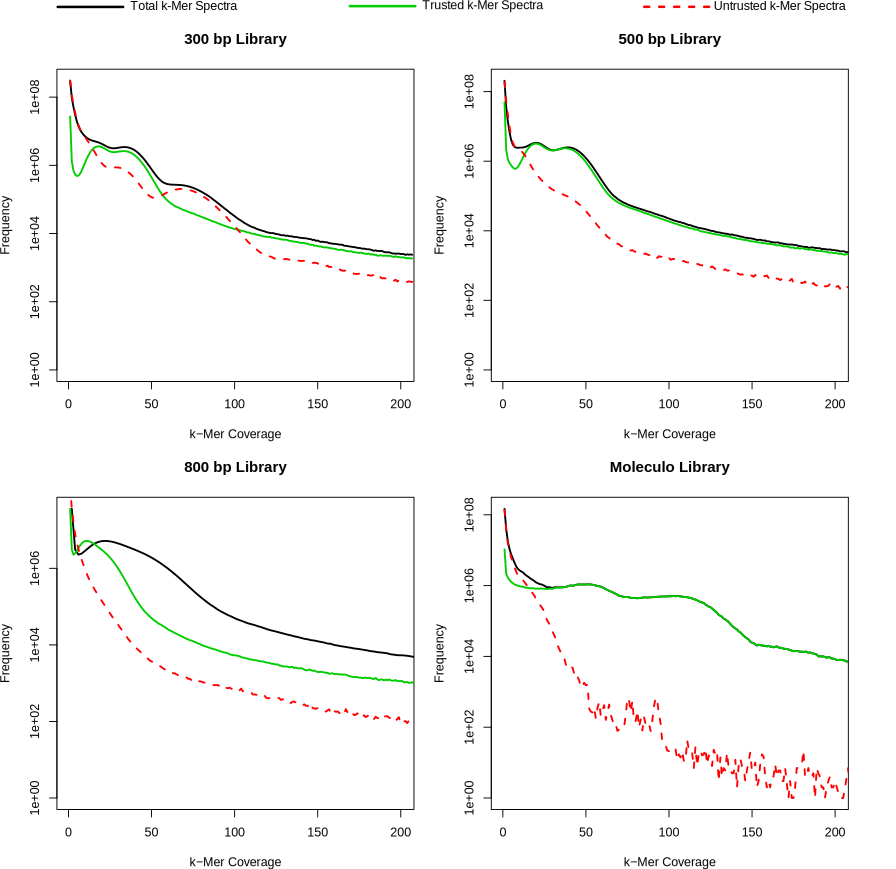
\includegraphics[width=1\textwidth]{supplementary_figure_1}
\captionof{figure}[kmer Analysis]{The plots depict the kmer
  distribution for each library before (black line) and after
  classification into ``trusted'' (green line) and ``untrusted'' kmers
  (red line).}

\pagebreak

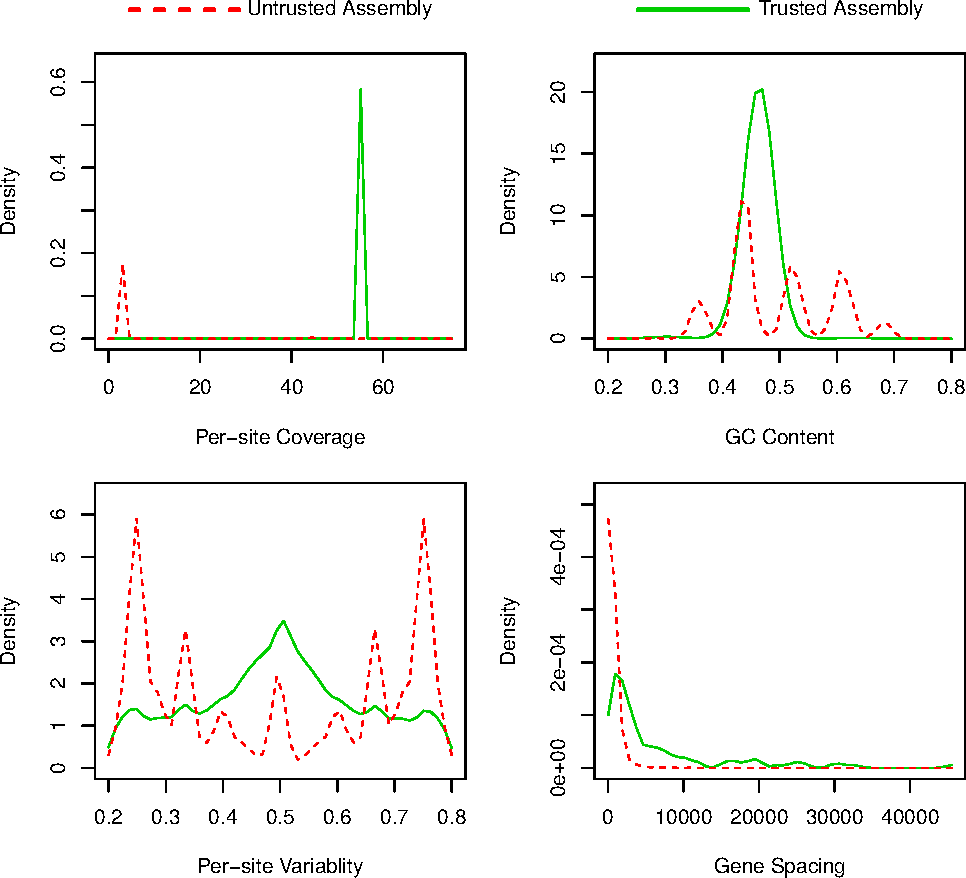
\includegraphics[width=1\textwidth]{supplementary_figure_2}
\captionof{figure}[Assembly Feature Comparisons]{A) Per-site coverage of trusted and untrusted assembly based on mappings of Moleculo reads. Contigs from the untrusted assembly generally don't share the coverage of the trusted, most likley nuclear, genome. B) GC concent of trusted and untrusted assembly estimated using sliding window approach. The untrusted assembly contains multiple peaks pointing towards contig subpopulations with different GC content. C) Per-site variability of trusted und untrusted assembly which can serve as ploidy proxy. The untrusted variability spectrum seems distored and contains a multiude of different peaks while the trusted assembly shows a typical diploid spectrum. D) Lenght distribution of intergenetic regions. Intragenetic regions are significantly larger in the trusted assembly than in the trusted.}

\pagebreak

\includegraphics[width=1\textwidth]{supplementary_figure_3}
\captionof{figure}[Unknown Bacterial Genome]{Circular map of an unknown bacterial genome probably belonging to the Chitinophagaceae drawn with CGView. Track 1 and 2 (blue) indicate GeneMark-S annoated genes on forward and reverse strand. Track 3 (red) visualizes regions of homology to a set of 30,844 Chitinophagaceae proteins downloaded from UniProtKB. Track 4 (green) shows homology between GeneMark-S predicted proteins and the published protein set of Boothby et al.}

\pagebreak

\section{Methods}

\subsection*{GitHub repository}
All script files are available from our GitHub repository (\url{https://github.com/greatfireball/hypsibius_genome_revised/}).

\subsection*{Data set}
We used the data set provided by \textcite{Boothby2015} and downloaded the data from \url{http://weatherby.genetics.utah.edu/seq_transf/}. A complete list of the used input files are given in \cref{tab:inputdata}.

\begin{sidewaystable}
\centering
\captionof{table}{\label{tab:inputdata}Bla}
\begin{tabularx}{\linewidth}{>{\ttfamily\tiny}X>{\ttfamily\tiny}l>{\ttfamily\tiny}r*{2}{>{\ttfamily\tiny}l}}\toprule
Filename and location                                          & Modification time    & Size in Bytes     & MD5 check sum                    & MD5 check sum decompressed \\ \midrule
\href{http://weatherby.genetics.utah.edu/seq_transf/tg.genome.fsa.gz}{tg.genome.fsa.gz}
                                                               & 2015-11-25T01:34:44Z &    \num{72215266} & b8bd39390ef35dd43d1cda1ca6944d5a & 77be374d28b91232c0810cc4d3cd37b9 \\
\href{http://weatherby.genetics.utah.edu/seq_transf/tg.default.maker.proteins.final.fasta.gz}{tg.default.maker.proteins.final.fasta.gz}
                                                               & 2015-12-02T23:43:44Z &    \num{12359873} & 2de12e5d28d6dba121973db2071565d9 & 1ad17cfa9e6c26e552fa8048c6ee90af \\
\href{http://weatherby.genetics.utah.edu/seq_transf/short_reads/TG-300-SIPE_1_sequence.txt}{short\_reads/TG-300-SIPE\_1\_sequence.txt}
                                                               & 2015-11-30T21:48:51Z & \num{11526955725} & c16b5442c9893b6feaa3aa81a39eefcd & c16b5442c9893b6feaa3aa81a39eefcd \\
\href{http://weatherby.genetics.utah.edu/seq_transf/short_reads/TG-300-SIPE_2_sequence.txt.gz}{short\_reads/TG-300-SIPE\_2\_sequence.txt.gz}
                                                               & 2015-11-30T21:52:41Z &  \num{3920224257} & 3bea43d66d71926fb620966d281598c6 & bc8423d4fe4275863e0809445ffd21ce \\
\href{http://weatherby.genetics.utah.edu/seq_transf/short_reads/TG-500-SIPE_1_sequence.txt.gz}{short\_reads/TG-500-SIPE\_1\_sequence.txt.gz}
                                                               & 2015-12-01T05:32:05Z &  \num{2738243219} & da8b15d388961938584343f8926f7b24 & eee7363557ccb1fb0fa75ebe55ae7ee5 \\
\href{http://weatherby.genetics.utah.edu/seq_transf/short_reads/TG-500-SIPE_2_sequence.txt.gz}{short\_reads/TG-500-SIPE\_2\_sequence.txt.gz}
                                                               & 2015-12-01T05:35:15Z &  \num{2805269168} & aa8c2c345484b9464d272e0993d6968b & 325d74bbafd9b6019609e2fd33eca260 \\
\href{http://weatherby.genetics.utah.edu/seq_transf/short_reads/TG-800-SIPE_1_sequence.txt.gz}{short\_reads/TG-800-SIPE\_1\_sequence.txt.gz}
                                                               & 2015-12-01T05:36:55Z &  \num{2155735304} & 6e9cce1a27000ae2b4f87181a976df92 & a85568ef53979c367870eee6390f2ced \\
\href{http://weatherby.genetics.utah.edu/seq_transf/short_reads/TG-800-SIPE_2_sequence.txt.gz}{short\_reads/TG-800-SIPE\_2\_sequence.txt.gz}
                                                               & 2015-12-01T05:37:46Z &  \num{2058207374} & ccf097cf4f13bb5cbc5a8e002250093d & 4a4cc02c2f289d59c300810fb621eb28 \\
\href{http://weatherby.genetics.utah.edu/seq_transf/moleculo_reads/LR6000049-DNA_A01-LRAAD-01_LongRead.fastq.gz}{moleculo\_reads/LR6000049-DNA\_A01-LRAAD-01\_LongRead.fastq.gz}
                                                               & 2015-11-30T17:50:17Z &   \num{825877986} & 86e75544f2d6ef5185bae419bbd2a4b2 & bace73ed4750b33fc144e56c155454ab \\
\href{http://weatherby.genetics.utah.edu/seq_transf/moleculo_reads/LR6000049-DNA_A01-LRAAD-02_LongRead.fastq.gz}{moleculo\_reads/LR6000049-DNA\_A01-LRAAD-02\_LongRead.fastq.gz}
                                                               & 2015-11-30T17:51:34Z &   \num{835283315} & 4dea3e39a7a25059a6ebbd5588e845b2 & cb83c39f9a385f0b4fd1e507cfe40ff1 \\
\href{http://weatherby.genetics.utah.edu/seq_transf/moleculo_reads/LR6000049-DNA_A01-LRAAD-03_LongRead.fastq.gz}{moleculo\_reads/LR6000049-DNA\_A01-LRAAD-03\_LongRead.fastq.gz}
                                                               & 2015-11-30T17:52:51Z &   \num{847867943} & 16276b6ef8dea90721eb67ac21d616e6 & 51d4ce37668684b4aa25e061fb95b4ef \\
\href{http://weatherby.genetics.utah.edu/seq_transf/moleculo_reads/LR6000049-DNA_A01-LRAAD-04_LongRead.fastq.gz}{moleculo\_reads/LR6000049-DNA\_A01-LRAAD-04\_LongRead.fastq.gz}
                                                               & 2015-11-30T17:56:08Z &   \num{859746540} & 3364040445c7377c9323f82d98a2258c & dbe06ec4248199f416bb1d02ff1e65f5 \\
\href{http://weatherby.genetics.utah.edu/seq_transf/moleculo_reads/LR6000049-DNA_A01-LRAAD-05_LongRead.fastq.gz}{moleculo\_reads/LR6000049-DNA\_A01-LRAAD-05\_LongRead.fastq.gz}
                                                               & 2015-11-30T17:56:51Z &   \num{854266597} & 7995559df803ef0de0250f1bfac71f1a & 98d30f3ceb813d9f53c6df2ed1fa2239 \\
\end{tabularx}
\end{sidewaystable}

\subsection*{Programs}

\captionof{table}{\label{tab:programs}List of all programs including the version numbers and references to publications or websites used for the data processing and analysis}
\begin{tabularx}{\linewidth}{llX}\toprule
Programname & Version & Reference \\ \midrule
Allpath-LG  & v\,50378 & \textcite{Gnerre2011, Ribeiro2012} \\
BEDTools    & v\,2.20.1 & \textcite{Quinlan2010} \\
bioperl     & v\,1.69.1 & \textcite{Stajich2002} \\
bowtie2     & v\,2.2.2 & \textcite{Langmead2012} \\
bwa         & v\,0.7.10 & \textcite{Li2009a,Li2010} \\
CGView      & v\,1.0 & \textcite{Grin2011} \\
Falcon      & v\,0.4.0 & \url{https://github.com/PacificBiosciences/falcon} \\
Genemark-S  & v\,4.3.2 & \textcite{Besemer2001} \\
Genemark-ET & v\,4.29 & \textcite{Lomsadze2014} \\
Jellyfish   & v\,2.2.4  & \textcite{Marcais2011} \\
Perl        & v\,5.14.2  & \url{https://www.perl.org/} \\
samtools    & v\,1.1 & \textcite{Li2009b, Li2011a, Li2011b} \\
skewer      & v\,0.1.124 & \textcite{Jiang2014} \\
Trimmomatic & v\,0.3.5 & \textcite{Bolger2014} \\
\end{tabularx}

\subsection*{Trimming of the input data}

Short reads were trimmed with skewer.

\begin{lstlisting}{language=bash}
skewer -m pe -q 30 -Q 30 -l 60 -t 64 \
   HD_gen.il_L[358]*00_P1.fastq HD_gen.il_L[358]*00_P2.fastq
\end{lstlisting}

Long reads were trimmed with Trimmomatic.

\begin{lstlisting}{language=bash}
java -jar trimmomatic-0.35.jar SE -phred33 HD_gen.mo_L[12345]*.fastq \
   HD_gen.mo_L[12345]*.trimmed.fastq \
   ILLUMINACLIP:adapter.fa:2:30:10 LEADING:30 TRAILING:30 MINLEN:250
\end{lstlisting}

\subsection*{Estimation of the genomes size}

The genome size was esitmated by running the standalone error correction pipeline of Allpahts-LG.

\begin{lstlisting}{language=bash}
ErrorCorrectReads.pl PHRED_ENCODING=33 READS_OUT=$OUT \
   KEEP_KMER_SPECTRA=1 MAX_MEMORY_GB=$MEM \
   PAIRED_READS_A_IN=$PE1 \
   PAIRED_READS_B_IN=$PE2 \
   THREADS=$CPU HAPLOIDIFY=TRUE
\end{lstlisting}

\subsection*{Counting and Filtering bases on kmers}

The kmers of all libraries where counted using the software jellyfish \parencite{Marcais2011}:

\begin{lstlisting}[language=bash]
./scripts/count_kmers.sh
\end{lstlisting}

The resulting kmer hashes need to be dumped and converted to a hash
utilized later during the filtering step. This step and the following
required \SI{>200}{\giga\byte} of memory and was performed by the perl
script \texttt{prepare\_filter\_fastq\_by\_valid\_kmers.pl}.

\begin{lstlisting}[language=bash]
./scripts/dump_kmers.sh
\end{lstlisting}

The generated hash was used to filter individual libraries by the perl
script \texttt{filter\_fastq\_by\_valid\_kmers\_reduced.pl}.

\begin{lstlisting}[language=bash]
./scripts/filter_input_data.sh
\end{lstlisting}

The filtered data sets are classified as ``trusted'' or ``untrusted''
based on the ``trusted'' kmer content. Reads with at least
\SI{95}{\percent} ``trusted'' kmers content are called ``trusted''
while reads below that threshold are classified as ``untrusted''.

\begin{lstlisting}[language=bash]
./scripts/extract_classified_sequences.sh
\end{lstlisting}

\subsection*{Long Read Assembly}

Trusted and untrusted Moleculo reads were assembled with Falcon.

\begin{lstlisting}[language=bash]
fc_run.py trusted.falcon.cfg
fc_run.py untrusted.falcon.cfg
\end{lstlisting}

See configuration files for parameter details.

\subsection*{Assembly Annotation}
The trusted assembly was annotated with GeneMark-ES.

\begin{lstlisting}[language=bash]
gmes_petap.pl --sequence HD_gen.trusted.fasta \
   --ES --cores 64
\end{lstlisting}

The untrusted assemmbly was annotated with GeneMark-S

\begin{lstlisting}[language=bash]
gmsn.pl --fnn --faa --species HD --gm \
   --name HD HD_gen.unsupported.fasta
\end{lstlisting}

The largest untrusted sequence was visualized using the CGView Server.

\subsection*{Assembly Comparison}

Trusted and untrusted assemblies were compared using GC content, mapping coverage, per-site variability and gene spacing.

\paragraph{GC content}
The GC content was determined for all contigs
\SI{\ge1}{\kilo\basepair} using a sliding window of
\SI{1}{\kilo\basepair} and a stepsize of \SI{100}{\basepair} by the
perl script \texttt{sliding\_window\_gc.pl}.

\begin{lstlisting}[language=bash]
mkdir cg
cd cg

for i in ../assemblies/HD*.fasta
do
   ../scripts/sliding_window_gc/sliding_window_gc.pl
      --in "$i" \
      --min-length 1000
      > $(basename "$i").sliding_gc.tsv
done
\end{lstlisting}

\paragraph{Mapping Coverage}
The mapping coverage was determinded by remapping of the short or
longreads onto the assembled contig. For the short read libraries, we
used \texttt{bowtie2} as mapper. Long read libraries were mapped by
\texttt{bwa}. The per-base coverage was determined by bedtools.

\begin{lstlisting}[language=bash]
mkdir mapping
cd mapping

BWA=bwa
SAMTOOLS=samtools

ln -s ../assemblies/HD*.fasta ./

# prepare mapping indices for bowtie2 and bwa
for i in *.fasta
do
   # bowtie2 preparation
   bowtie2-build "$i" \
      $(basename "$i" .fasta) 2>&1 | \
      tee bowtie2-build-$(basename "$i" .fasta).log
   # bwa preparation
   bwa index "$i" 2>&1 | \
      tee bwa-index-$(basename "$i" .fasta).log
done

# mapping of short reads
for REF in HD_gen.supported.fasta HD_gen.unsupported.fasta
do
   # 300 bp library
   bowtie2 \
        -x "$REF" \
        -1 ../trimmed/HD_gen.il_L300.trimmed_P1.fastq \
        -2 ../trimmed/HD_gen.il_L300.trimmed_P2.fastq \
        -p 32 \
        --minins 0 \
        --maxins 900 | \
        samtools view -uS - | \
        samtools sort -@32 - "$REF"-il.L300

   # 500 bp library
   bowtie2 \
        -x "$REF" \
        -1 ../trimmed/HD_gen.il_L500.trimmed_P1.fastq \
        -2 ../trimmed/HD_gen.il_L500.trimmed_P2.fastq \
        -p 32 \
        --minins 0 \
        --maxins 1500 | \
        samtools view -uS - | \
        samtools sort -@32 - "$REF"-il.L500

   # 800 bp library
   bowtie2 \
        -x "$REF" \
        -1 ../trimmed/HD_gen.il_L800.trimmed_P1.fastq \
        -2 ../trimmed/HD_gen.il_L800.trimmed_P2.fastq \
        -p 32 \
        --minins 0 \
        --maxins 2400 | \
        samtools view -uS - | \
        samtools sort -@32 - "$REF"-il.L800
done

# mapping of long reads
# combine all long reads
find ../trimmed/ -name "HD_gen.mo_L[12345].trimmed.formatted.fastq" | \
   xargs cat > ../trimmed/HD_gen.mo_L12345.trimmed.formatted.fastq

# map the longreads
for REF in HD_gen.supported.fasta HD_gen.unsupported.fasta
do
   for SEQ in ../trimmed/HD_gen.mo_L12345.trimmed.formatted.fastq
      OUT=$(basename "$REF")_$(basename "$SEQ")

      $BWA mem -t 32 "$REF" "$SEQ" | \
      $SAMTOOLS view -uS - | \
      $SAMTOOLS sort -@32 - "$OUT"
   done
done

# extraction of per base coverage
for REF in HD_gen.supported.fasta HD_gen.unsupported.fasta
do
   for BAM in "$REF"*.bam
   do
      OUT=$(basename "$BAM" .bam).cov
      bedtools genomecov \
         -ibam "$BAM" -d -g "$REF" > "$OUT"
   done
done
\end{lstlisting}

\paragraph{per-site Variability}

The per-site variablity was calculated by counting bases covering each site of the two assembly. Each base that occurred at a given site with a minimum frequency of 0.2 was taken into account and a histogram of all these base frequencies was created.

\paragraph{Gene Spacing}

Lenght of the intragenetic regions were directly extracted from the GeneMark-S/ES annotation files.

\begin{lstlisting}[language=bash]
gtf2genespacing.pl --gtf HD_gen.supported.gtf 
gtf2genespacing.pl --gtf HD_gen.unsupported.gtf
\end{lstlisting}

All resulting data set were compared, tested and visualized using the GNU R package 'sm'.

\printbibliography

\end{document}
